\documentclass[]{article}
\usepackage{lmodern}
\usepackage{amssymb,amsmath}
\usepackage{ifxetex,ifluatex}
\usepackage{fixltx2e} % provides \textsubscript
\ifnum 0\ifxetex 1\fi\ifluatex 1\fi=0 % if pdftex
  \usepackage[T1]{fontenc}
  \usepackage[utf8]{inputenc}
\else % if luatex or xelatex
  \ifxetex
    \usepackage{mathspec}
  \else
    \usepackage{fontspec}
  \fi
  \defaultfontfeatures{Ligatures=TeX,Scale=MatchLowercase}
\fi
% use upquote if available, for straight quotes in verbatim environments
\IfFileExists{upquote.sty}{\usepackage{upquote}}{}
% use microtype if available
\IfFileExists{microtype.sty}{%
\usepackage{microtype}
\UseMicrotypeSet[protrusion]{basicmath} % disable protrusion for tt fonts
}{}
\usepackage[margin=1in]{geometry}
\usepackage{hyperref}
\hypersetup{unicode=true,
            pdftitle={Filtering Raw Data},
            pdfauthor={Hayden Green},
            pdfborder={0 0 0},
            breaklinks=true}
\urlstyle{same}  % don't use monospace font for urls
\usepackage{color}
\usepackage{fancyvrb}
\newcommand{\VerbBar}{|}
\newcommand{\VERB}{\Verb[commandchars=\\\{\}]}
\DefineVerbatimEnvironment{Highlighting}{Verbatim}{commandchars=\\\{\}}
% Add ',fontsize=\small' for more characters per line
\usepackage{framed}
\definecolor{shadecolor}{RGB}{248,248,248}
\newenvironment{Shaded}{\begin{snugshade}}{\end{snugshade}}
\newcommand{\AlertTok}[1]{\textcolor[rgb]{0.94,0.16,0.16}{#1}}
\newcommand{\AnnotationTok}[1]{\textcolor[rgb]{0.56,0.35,0.01}{\textbf{\textit{#1}}}}
\newcommand{\AttributeTok}[1]{\textcolor[rgb]{0.77,0.63,0.00}{#1}}
\newcommand{\BaseNTok}[1]{\textcolor[rgb]{0.00,0.00,0.81}{#1}}
\newcommand{\BuiltInTok}[1]{#1}
\newcommand{\CharTok}[1]{\textcolor[rgb]{0.31,0.60,0.02}{#1}}
\newcommand{\CommentTok}[1]{\textcolor[rgb]{0.56,0.35,0.01}{\textit{#1}}}
\newcommand{\CommentVarTok}[1]{\textcolor[rgb]{0.56,0.35,0.01}{\textbf{\textit{#1}}}}
\newcommand{\ConstantTok}[1]{\textcolor[rgb]{0.00,0.00,0.00}{#1}}
\newcommand{\ControlFlowTok}[1]{\textcolor[rgb]{0.13,0.29,0.53}{\textbf{#1}}}
\newcommand{\DataTypeTok}[1]{\textcolor[rgb]{0.13,0.29,0.53}{#1}}
\newcommand{\DecValTok}[1]{\textcolor[rgb]{0.00,0.00,0.81}{#1}}
\newcommand{\DocumentationTok}[1]{\textcolor[rgb]{0.56,0.35,0.01}{\textbf{\textit{#1}}}}
\newcommand{\ErrorTok}[1]{\textcolor[rgb]{0.64,0.00,0.00}{\textbf{#1}}}
\newcommand{\ExtensionTok}[1]{#1}
\newcommand{\FloatTok}[1]{\textcolor[rgb]{0.00,0.00,0.81}{#1}}
\newcommand{\FunctionTok}[1]{\textcolor[rgb]{0.00,0.00,0.00}{#1}}
\newcommand{\ImportTok}[1]{#1}
\newcommand{\InformationTok}[1]{\textcolor[rgb]{0.56,0.35,0.01}{\textbf{\textit{#1}}}}
\newcommand{\KeywordTok}[1]{\textcolor[rgb]{0.13,0.29,0.53}{\textbf{#1}}}
\newcommand{\NormalTok}[1]{#1}
\newcommand{\OperatorTok}[1]{\textcolor[rgb]{0.81,0.36,0.00}{\textbf{#1}}}
\newcommand{\OtherTok}[1]{\textcolor[rgb]{0.56,0.35,0.01}{#1}}
\newcommand{\PreprocessorTok}[1]{\textcolor[rgb]{0.56,0.35,0.01}{\textit{#1}}}
\newcommand{\RegionMarkerTok}[1]{#1}
\newcommand{\SpecialCharTok}[1]{\textcolor[rgb]{0.00,0.00,0.00}{#1}}
\newcommand{\SpecialStringTok}[1]{\textcolor[rgb]{0.31,0.60,0.02}{#1}}
\newcommand{\StringTok}[1]{\textcolor[rgb]{0.31,0.60,0.02}{#1}}
\newcommand{\VariableTok}[1]{\textcolor[rgb]{0.00,0.00,0.00}{#1}}
\newcommand{\VerbatimStringTok}[1]{\textcolor[rgb]{0.31,0.60,0.02}{#1}}
\newcommand{\WarningTok}[1]{\textcolor[rgb]{0.56,0.35,0.01}{\textbf{\textit{#1}}}}
\usepackage{graphicx,grffile}
\makeatletter
\def\maxwidth{\ifdim\Gin@nat@width>\linewidth\linewidth\else\Gin@nat@width\fi}
\def\maxheight{\ifdim\Gin@nat@height>\textheight\textheight\else\Gin@nat@height\fi}
\makeatother
% Scale images if necessary, so that they will not overflow the page
% margins by default, and it is still possible to overwrite the defaults
% using explicit options in \includegraphics[width, height, ...]{}
\setkeys{Gin}{width=\maxwidth,height=\maxheight,keepaspectratio}
\IfFileExists{parskip.sty}{%
\usepackage{parskip}
}{% else
\setlength{\parindent}{0pt}
\setlength{\parskip}{6pt plus 2pt minus 1pt}
}
\setlength{\emergencystretch}{3em}  % prevent overfull lines
\providecommand{\tightlist}{%
  \setlength{\itemsep}{0pt}\setlength{\parskip}{0pt}}
\setcounter{secnumdepth}{0}
% Redefines (sub)paragraphs to behave more like sections
\ifx\paragraph\undefined\else
\let\oldparagraph\paragraph
\renewcommand{\paragraph}[1]{\oldparagraph{#1}\mbox{}}
\fi
\ifx\subparagraph\undefined\else
\let\oldsubparagraph\subparagraph
\renewcommand{\subparagraph}[1]{\oldsubparagraph{#1}\mbox{}}
\fi

%%% Use protect on footnotes to avoid problems with footnotes in titles
\let\rmarkdownfootnote\footnote%
\def\footnote{\protect\rmarkdownfootnote}

%%% Change title format to be more compact
\usepackage{titling}

% Create subtitle command for use in maketitle
\providecommand{\subtitle}[1]{
  \posttitle{
    \begin{center}\large#1\end{center}
    }
}

\setlength{\droptitle}{-2em}

  \title{Filtering Raw Data}
    \pretitle{\vspace{\droptitle}\centering\huge}
  \posttitle{\par}
    \author{Hayden Green}
    \preauthor{\centering\large\emph}
  \postauthor{\par}
      \predate{\centering\large\emph}
  \postdate{\par}
    \date{9 April 2019}


\begin{document}
\maketitle

\begin{Shaded}
\begin{Highlighting}[]
\CommentTok{# Reading a fresh raw CSV file}

\NormalTok{list_of_checked_files <-}\StringTok{ }\KeywordTok{list.files}\NormalTok{(}\DataTypeTok{path =} \StringTok{"G:}\CharTok{\textbackslash{}\textbackslash{}}\StringTok{Team Drives}\CharTok{\textbackslash{}\textbackslash{}}\StringTok{Research Team}\CharTok{\textbackslash{}\textbackslash{}}\StringTok{Projects}\CharTok{\textbackslash{}\textbackslash{}}\StringTok{2018 Driving Sim Reproducibility}\CharTok{\textbackslash{}\textbackslash{}}\StringTok{7_Filtered_data}\CharTok{\textbackslash{}\textbackslash{}}\StringTok{"}\NormalTok{, }
                                    \DataTypeTok{pattern =} \StringTok{"*_checked.csv"}\NormalTok{, }\DataTypeTok{full.names =} \OtherTok{TRUE}\NormalTok{)}


\NormalTok{checked_csv <-}\StringTok{ }\KeywordTok{read_csv}\NormalTok{(list_of_checked_files[}\DecValTok{1}\NormalTok{])}
\end{Highlighting}
\end{Shaded}

\begin{verbatim}
## Parsed with column specification:
## cols(
##   .default = col_double(),
##   System_Time = col_character(),
##   ID = col_character(),
##   Date = col_date(format = ""),
##   session = col_logical(),
##   scenario = col_character()
## )
\end{verbatim}

\begin{verbatim}
## See spec(...) for full column specifications.
\end{verbatim}

\begin{Shaded}
\begin{Highlighting}[]
\NormalTok{unfiltered_speed_plot <-}\StringTok{ }\NormalTok{checked_csv }\OperatorTok\StringTok{ }
\StringTok{                         }\KeywordTok{ggplot}\NormalTok{(}\KeywordTok{aes}\NormalTok{(}\DataTypeTok{x=}\NormalTok{ Total_dist, }\DataTypeTok{y =}\NormalTok{ Speed)) }\OperatorTok{+}\StringTok{ }
\StringTok{                         }\KeywordTok{geom_line}\NormalTok{() }\OperatorTok{+}
\StringTok{                         }\KeywordTok{ylim}\NormalTok{(}\DecValTok{90}\NormalTok{,}\DecValTok{110}\NormalTok{)}\OperatorTok{+}
\StringTok{                         }\KeywordTok{theme_classic}\NormalTok{()}
\NormalTok{unfiltered_speed_plot}
\end{Highlighting}
\end{Shaded}

\begin{verbatim}
## Warning: Removed 479 rows containing missing values (geom_path).
\end{verbatim}

\includegraphics{Filtering_Raw_Drivesim_Data_files/figure-latex/unnamed-chunk-1-1.pdf}

\begin{Shaded}
\begin{Highlighting}[]
\NormalTok{unfiltered_lanepos_plot <-}\StringTok{ }\NormalTok{checked_csv }\OperatorTok\StringTok{ }
\StringTok{                         }\KeywordTok{ggplot}\NormalTok{(}\KeywordTok{aes}\NormalTok{(}\DataTypeTok{x=}\NormalTok{ Total_dist, }\DataTypeTok{y =}\NormalTok{ Lateral_Lane_Pos }\OperatorTok{+}\DecValTok{6}\NormalTok{)) }\OperatorTok{+}\StringTok{ }
\StringTok{                         }\KeywordTok{geom_line}\NormalTok{() }\OperatorTok{+}
\StringTok{                         }\KeywordTok{ylab}\NormalTok{(}\StringTok{"Lateral Lane Position (m)"}\NormalTok{)}\OperatorTok{+}
\StringTok{                         }\KeywordTok{theme_classic}\NormalTok{()}
\NormalTok{unfiltered_lanepos_plot}
\end{Highlighting}
\end{Shaded}

\includegraphics{Filtering_Raw_Drivesim_Data_files/figure-latex/unnamed-chunk-1-2.pdf}

\begin{Shaded}
\begin{Highlighting}[]
\CommentTok{#checked_csv %>% mutate(filtered_speed = FilterOfOrder(n = 1, x = Speed, type = "high", Wc = 0.1 ))}

\CommentTok{#filt_speed_plot <- checked_csv %>% fil() }
\NormalTok{binned_csv <-}\StringTok{ }\KeywordTok{read_csv}\NormalTok{(}\StringTok{"G:}\CharTok{\textbackslash{}\textbackslash{}}\StringTok{Team Drives}\CharTok{\textbackslash{}\textbackslash{}}\StringTok{Research Team}\CharTok{\textbackslash{}\textbackslash{}}\StringTok{Projects}\CharTok{\textbackslash{}\textbackslash{}}\StringTok{2018 Driving Sim Reproducibility}\CharTok{\textbackslash{}\textbackslash{}}\StringTok{4_Analysis_Saccades}\CharTok{\textbackslash{}\textbackslash{}}\StringTok{AL}\CharTok{\textbackslash{}\textbackslash{}}\StringTok{Session 1}\CharTok{\textbackslash{}\textbackslash{}}\StringTok{AL_10_binned_by_dist_100.csv"}\NormalTok{)}
\end{Highlighting}
\end{Shaded}

\begin{verbatim}
## Parsed with column specification:
## cols(
##   .default = col_double(),
##   ID = col_character(),
##   Date = col_date(format = ""),
##   Scenario = col_character()
## )
## See spec(...) for full column specifications.
\end{verbatim}

\begin{Shaded}
\begin{Highlighting}[]
\NormalTok{binned_csv <-}\StringTok{ }\NormalTok{binned_csv }\OperatorTok\StringTok{ }\NormalTok{dplyr}\OperatorTok{::}\KeywordTok{filter}\NormalTok{(}\StringTok{`}\DataTypeTok{bin_number}\StringTok{`} \OperatorTok{<}\StringTok{ }\DecValTok{301}\NormalTok{)}

\KeywordTok{mean}\NormalTok{(checked_csv}\OperatorTok{$}\NormalTok{Speed)}
\end{Highlighting}
\end{Shaded}

\begin{verbatim}
## [1] 97.75934
\end{verbatim}

\begin{Shaded}
\begin{Highlighting}[]
\KeywordTok{sd}\NormalTok{(checked_csv}\OperatorTok{$}\NormalTok{Speed)}
\end{Highlighting}
\end{Shaded}

\begin{verbatim}
## [1] 3.615161
\end{verbatim}

\begin{Shaded}
\begin{Highlighting}[]
\KeywordTok{mean}\NormalTok{(checked_csv}\OperatorTok{$}\NormalTok{Lateral_Lane_Pos}\OperatorTok{+}\DecValTok{6}\NormalTok{)}
\end{Highlighting}
\end{Shaded}

\begin{verbatim}
## [1] 0.0797916
\end{verbatim}

\begin{Shaded}
\begin{Highlighting}[]
\KeywordTok{sd}\NormalTok{(checked_csv}\OperatorTok{$}\NormalTok{Lateral_Lane_Pos}\OperatorTok{+}\DecValTok{6}\NormalTok{)}
\end{Highlighting}
\end{Shaded}

\begin{verbatim}
## [1] 1.649434
\end{verbatim}

\begin{Shaded}
\begin{Highlighting}[]
\KeywordTok{mean}\NormalTok{(binned_csv}\OperatorTok{$}\NormalTok{sd_speed)}
\end{Highlighting}
\end{Shaded}

\begin{verbatim}
## [1] 0.1917473
\end{verbatim}

\begin{Shaded}
\begin{Highlighting}[]
\KeywordTok{sd}\NormalTok{(binned_csv}\OperatorTok{$}\NormalTok{avg_speed)}
\end{Highlighting}
\end{Shaded}

\begin{verbatim}
## [1] 2.166878
\end{verbatim}

\begin{Shaded}
\begin{Highlighting}[]
\KeywordTok{mean}\NormalTok{(binned_csv}\OperatorTok{$}\NormalTok{sd_lanepos)}
\end{Highlighting}
\end{Shaded}

\begin{verbatim}
## [1] 0.4652335
\end{verbatim}

\begin{Shaded}
\begin{Highlighting}[]
\KeywordTok{sd}\NormalTok{(binned_csv}\OperatorTok{$}\NormalTok{avg_lanepos}\OperatorTok{+}\DecValTok{6}\NormalTok{)}
\end{Highlighting}
\end{Shaded}

\begin{verbatim}
## [1] 1.554944
\end{verbatim}

\hypertarget{filtering-the-data}{%
\section{Filtering the data}\label{filtering-the-data}}

\begin{Shaded}
\begin{Highlighting}[]
\CommentTok{#Setting the parameteres of the highpass filter (first order, 0.1Hz)}
\NormalTok{bfhigh <-}\StringTok{ }\KeywordTok{butter}\NormalTok{(}\DecValTok{1}\NormalTok{, }\KeywordTok{c}\NormalTok{(}\DecValTok{0}\NormalTok{,}\FloatTok{0.1}\NormalTok{), }\DataTypeTok{type =} \StringTok{"high"}\NormalTok{)}
\NormalTok{checked_csv <-}\StringTok{ }\NormalTok{checked_csv }\OperatorTok
\StringTok{               }\NormalTok{dplyr}\OperatorTok{::}\KeywordTok{filter}\NormalTok{(Total_dist }\OperatorTok{>}\StringTok{ }\DecValTok{900}\NormalTok{) }\OperatorTok\StringTok{ }
\StringTok{               }\KeywordTok{mutate}\NormalTok{(}\DataTypeTok{filtered_speed =} \KeywordTok{filter}\NormalTok{(bfhigh,Speed), }\DataTypeTok{filtered_lane_pos =} \KeywordTok{filter}\NormalTok{(bfhigh,Lateral_Lane_Pos }\OperatorTok{+}\StringTok{ }\DecValTok{6}\NormalTok{))}

\NormalTok{filtered_speed_plot <-}\StringTok{ }\NormalTok{checked_csv }\OperatorTok\StringTok{ }
\StringTok{                         }\KeywordTok{ggplot}\NormalTok{(}\KeywordTok{aes}\NormalTok{(}\DataTypeTok{x=}\NormalTok{ Total_dist, }\DataTypeTok{y =}\NormalTok{ filtered_speed)) }\OperatorTok{+}\StringTok{ }
\StringTok{                         }\KeywordTok{geom_line}\NormalTok{() }\OperatorTok{+}
\StringTok{                         }\KeywordTok{ylim}\NormalTok{(}\OperatorTok{-}\DecValTok{1}\NormalTok{,}\DecValTok{1}\NormalTok{) }\OperatorTok{+}
\StringTok{                         }\KeywordTok{theme_classic}\NormalTok{()}


\NormalTok{filtered_lanepos_plot <-}\StringTok{ }\NormalTok{checked_csv }\OperatorTok\StringTok{ }
\StringTok{                         }\KeywordTok{ggplot}\NormalTok{(}\KeywordTok{aes}\NormalTok{(}\DataTypeTok{x=}\NormalTok{ Total_dist, }\DataTypeTok{y =}\NormalTok{ filtered_lane_pos)) }\OperatorTok{+}\StringTok{ }
\StringTok{                         }\KeywordTok{geom_line}\NormalTok{() }\OperatorTok{+}
\StringTok{                         }\KeywordTok{ylab}\NormalTok{(}\StringTok{"Lateral Lane Position (m)"}\NormalTok{)}\OperatorTok{+}
\StringTok{                         }\KeywordTok{theme_classic}\NormalTok{()}


\KeywordTok{plot_grid}\NormalTok{(unfiltered_lanepos_plot, filtered_lanepos_plot, }\DataTypeTok{labels =}  \KeywordTok{c}\NormalTok{(}\StringTok{"Lane Pos Unfiltered"}\NormalTok{,}\StringTok{"Lane Pos 0.1HZ Filtered"}\NormalTok{), }\DataTypeTok{scale =} \DecValTok{1}\NormalTok{)}
\end{Highlighting}
\end{Shaded}

\begin{verbatim}
## Don't know how to automatically pick scale for object of type ts. Defaulting to continuous.
\end{verbatim}

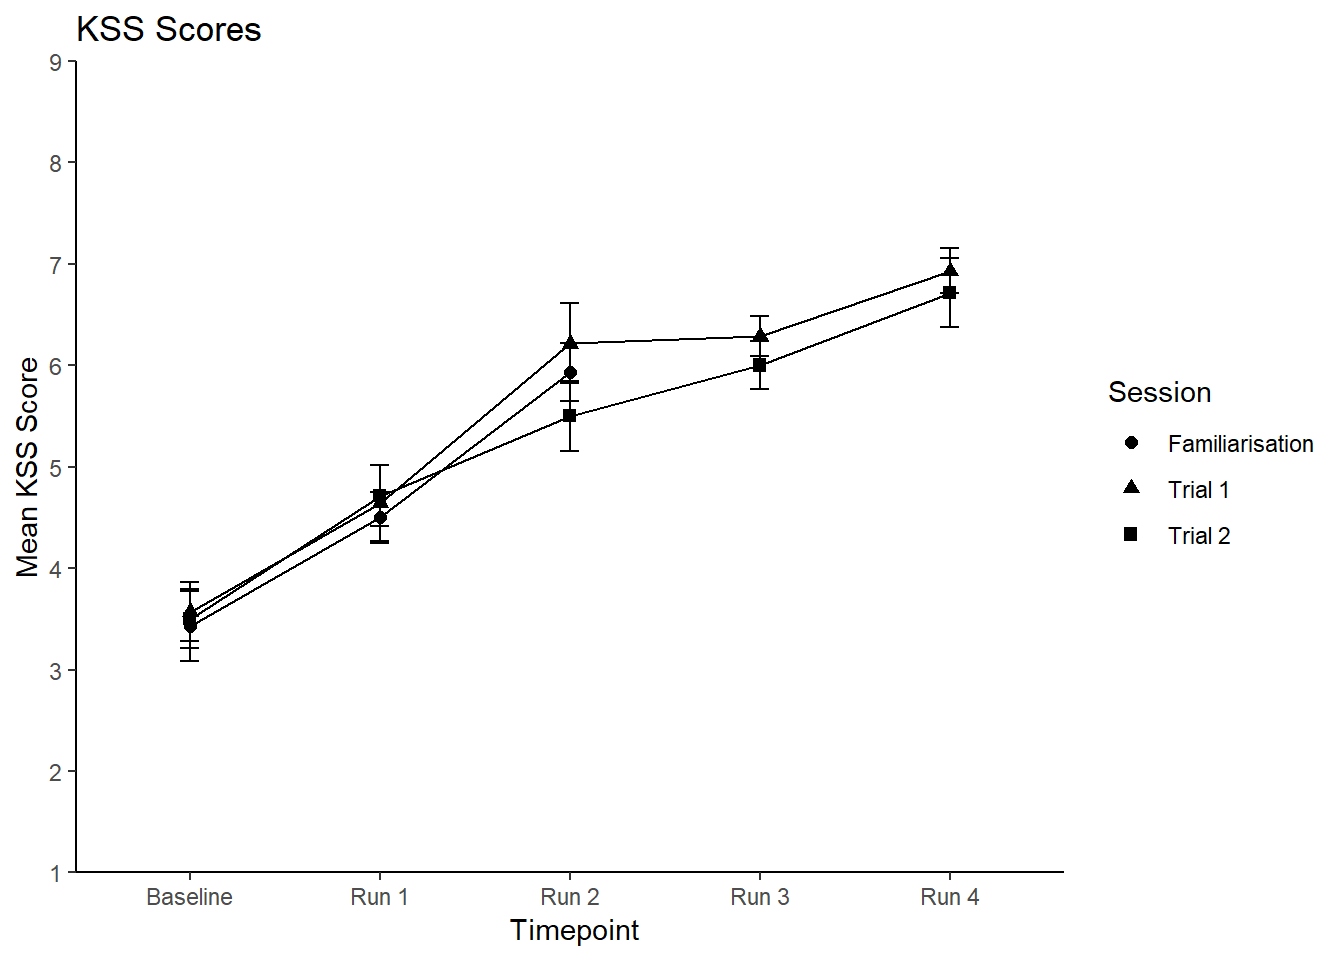
\includegraphics{Filtering_Raw_Drivesim_Data_files/figure-latex/unnamed-chunk-2-1.pdf}

\begin{Shaded}
\begin{Highlighting}[]
\KeywordTok{plot_grid}\NormalTok{(unfiltered_speed_plot, filtered_speed_plot, }\DataTypeTok{labels =}  \KeywordTok{c}\NormalTok{(}\StringTok{"Speed Unfiltered"}\NormalTok{,}\StringTok{"0.1HZ Filtered"}\NormalTok{), }\DataTypeTok{scale =} \DecValTok{1}\NormalTok{)}
\end{Highlighting}
\end{Shaded}

\begin{verbatim}
## Warning: Removed 479 rows containing missing values (geom_path).
\end{verbatim}

\begin{verbatim}
## Warning: Removed 14 rows containing missing values (geom_path).
\end{verbatim}

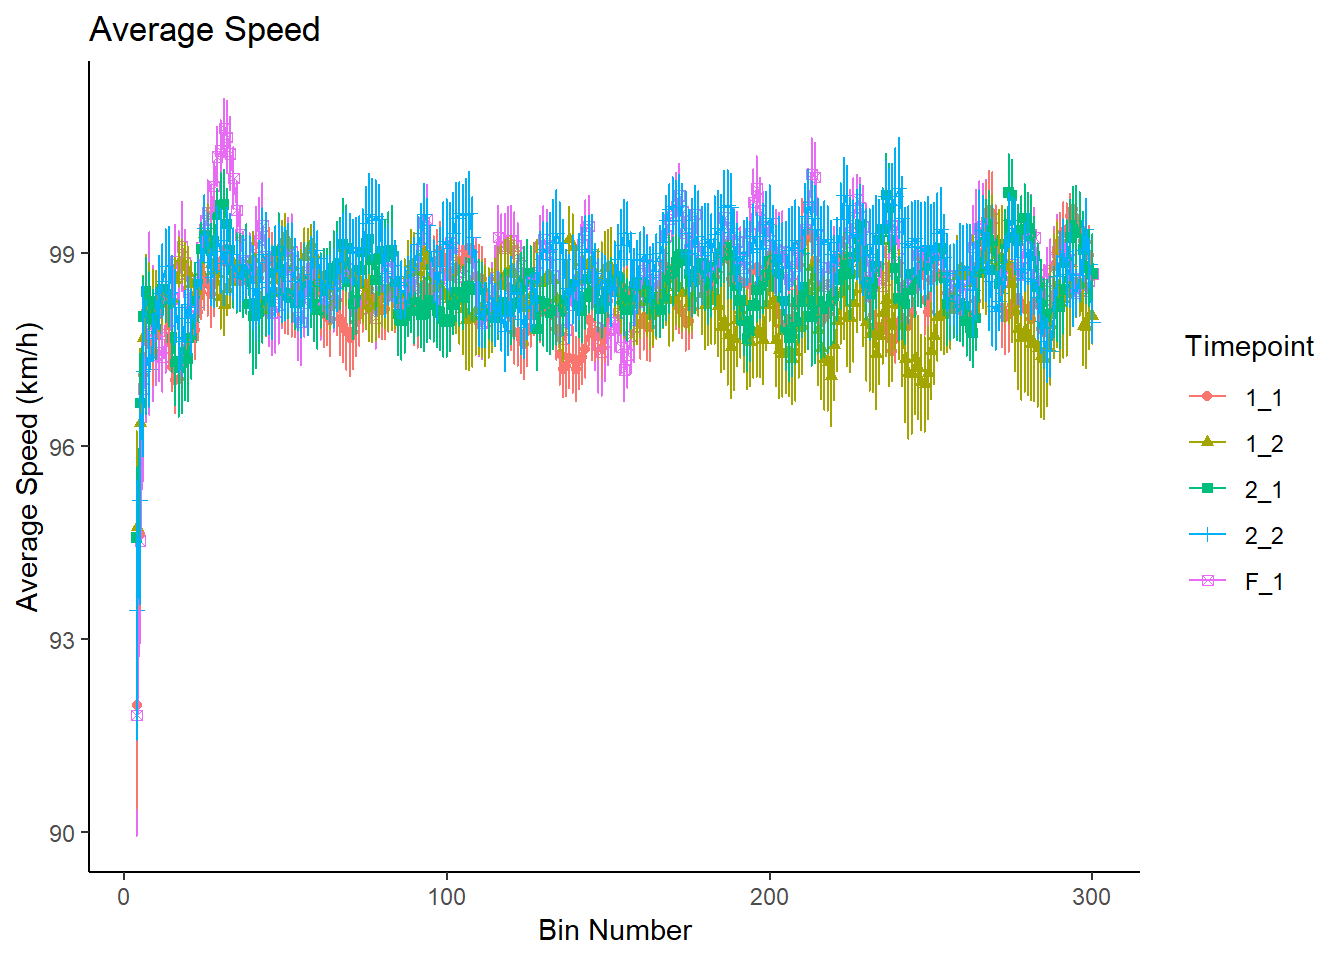
\includegraphics{Filtering_Raw_Drivesim_Data_files/figure-latex/unnamed-chunk-3-1.pdf}


\end{document}
